\documentclass{standalone}
\usepackage{pgfplots,xcolor}
\usepackage{amsmath,pgffor}
\usetikzlibrary{positioning,calc}
\pgfplotsset{compat=1.18}
\begin{document}

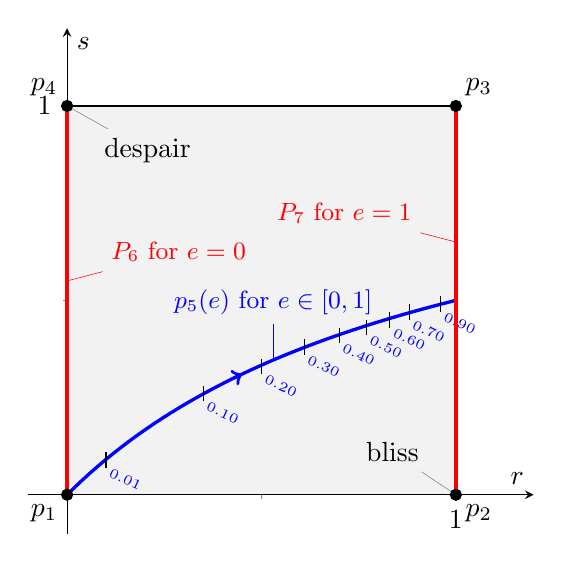
\begin{tikzpicture}
  \begin{axis}[
    axis equal image,
    xmin=-0.1, xmax=1.2,
    ymin=-0.1, ymax=1.2,
    axis lines=middle,
    xtick={0,1}, ytick={0,1},
    width=8cm, height=8cm,
    % grid=both,
    minor tick num=1,
    xlabel={$r$}, ylabel={$s$},
    ]
    \addplot [black, fill=gray!10] coordinates {(0,0) (1,0) (1,1)
      (0,1) (0,0)};
    
    \addplot[only marks,mark=*] coordinates {(0,0)};
    \node[anchor=north east] at (axis cs:0,0) {$p_1$};
    \addplot[only marks,mark=*] coordinates {(1,0)};
    \node[anchor=north west] at (axis cs:1,0) {$p_2$};
    \addplot[only marks,mark=*] coordinates {(1,1)};
    \node[anchor=south west] at (axis cs:1,1) {$p_3$};
    \addplot[only marks,mark=*] coordinates {(0,1)};
    \node[anchor=south east] at (axis cs:0,1) {$p_4$};

    %% p5 (arc)
    \addplot[very thick, domain=0:1,samples=50, blue, variable=x]
    (x, {x/(1+x)}) ;
    \node[coordinate, pin={[pin edge={blue}, blue, font=\small]90:{$p_5(e)$ for $e\in[0,1]$ }}] at
    (axis cs: 0.53, {0.53/(1+0.53)}) {};
    %%
    \node[coordinate] (p5_1) at
    (axis cs: 0.43, {0.43/(1+0.43)}) {};
    \node[coordinate] (p5_2) at
    (axis cs: 0.45, {0.45/(1+0.45)}) {};
    \draw[->, very thick, blue] (p5_1) -- (p5_2);
    \foreach
    \r / \x / \y in {%
      0.01 / 0.10 / 0.09,
      0.10 /  0.35 / 0.26,
      0.20 /  0.50 / 0.33,
      0.30 /  0.61 / 0.38,
      0.40 / 0.70 / 0.41,
      0.50 / 0.77 / 0.43,
      0.60 / 0.83 / 0.45,
      0.70 / 0.88 / 0.47,
      0.90 / 0.96 / 0.49
    }{%
      \edef\temp{
        \noexpand\node[rotate=-25, node font=\noexpand\tiny, blue] at (axis cs: \x+.05, \y-.05) {\r};
        \noexpand\draw (axis cs: \x, \y-.02 ) -- (axis cs: \x, \y+.02);
      }%
      \temp
    }

    %% P6 (links)
    \addplot[very thick, domain=0:1,samples=50, red, variable=s]
    (0,s);
    \node[coordinate, pin={[pin edge={red}, red, font=\small]15:{$P_{6}$ for $e=0$}}] (p6) at
    (axis cs: 0,0.55) {};
    
    %% P7 (rechts)
    \addplot[very thick, domain=0:1,samples=50, red, variable=s]
    (1,s);
    \node[coordinate, pin={[pin edge={red}, red, font=\small]165:{$P_{7}$ for $e=1$}}] (p7) at
    (axis cs: 1,0.65) {};


    \node[coordinate, pin=140:{bliss}] at (axis cs: 1,0) {};
    \node[coordinate, pin=-40:{despair}] at (axis cs: 0,1) {};

  \end{axis}
\end{tikzpicture}

\end{document}
